\documentclass[12pt,letterpaper]{article}
\usepackage[utf8]{inputenc}
\usepackage[spanish]{babel}
\usepackage{graphicx}
\usepackage[left=2cm,right=2cm,top=2cm,bottom=2cm]{geometry}
\usepackage{graphicx} % figuras
% \usepackage{subfigure} % subfiguras
\usepackage{float} % para usar [H]
\usepackage{amsmath}
%\usepackage{txfonts}
\usepackage{stackrel} 
\usepackage{multirow}
\usepackage{enumerate} % enumerados
\renewcommand{\labelitemi}{$-$}
\renewcommand{\labelitemii}{$\cdot$}
% \author{}
% \title{Caratula}
\begin{document}

% Fancy Header and Footer
% \usepackage{fancyhdr}
% \pagestyle{fancy}
% \cfoot{}
% \rfoot{\thepage}
%

% \usepackage[hidelinks]{hyperref} % CREA HYPERVINCULOS EN INDICE

% \author{}
\title{Caratula}

\begin{titlepage}
\begin{center}
\large{UNERSIDAD PRIVADA DE TACNA}\\
\vspace*{-0.025in}
\begin{figure}[htb]
\begin{center}

\includegraphics[width=8cm]{./Imagenes/logo}
\end{center}
\end{figure}
\vspace*{0.15in}
INGENIERIA DE SISTEMAS  \\

\vspace*{0.5in}
\begin{large}
TITULO:\\
\end{large}

\vspace*{0.1in}
\begin{Large}
\textbf{INFORME DE LABORATORIO No 01} \\
\end{Large}

\vspace*{0.3in}
\begin{Large}
\textbf{CURSO:} \\
\end{Large}

\vspace*{0.1in}
\begin{large}
BASE DE DATOS II\\
\end{large}

\vspace*{0.3in}
\begin{Large}
\textbf{DOCENTE(ING):} \\
\end{Large}

\vspace*{0.1in}
\begin{large}
 Patrick Cuadros Quiroga\\
\end{large}

\vspace*{0.2in}
\vspace*{0.1in}
\begin{large}
Integrantes: \\
\begin{flushleft}
Alfaro Musaja Jhosmell 	\hfill	(2015053223) \\
Katerin Merino Quispe 	\hfill	(2018060918) \\
Guimer Coaquira Coaquira 	\hfill	(2015053226) \\
\end{flushleft}
\end{large}
\end{center}

\end{titlepage}


\tableofcontents % INDICE
\thispagestyle{empty} % INDICE SIN NUMERO
\newpage
\setcounter{page}{1} % REINICIAR CONTADOR DE PAGINAS DESPUES DEL INDICE

\section{Actividad No 01 – Revisi\'on de Sintaxis} 
De los siguientes comandos ¿Cuál es el resultado? ¿En caso de ser error cual sería la sentencia correcta?

\begin{itemize}
	\item SELECT last\_name, job\_id, salary AS Sal FROM employees;
	\\Es correcta
	\begin{center}
	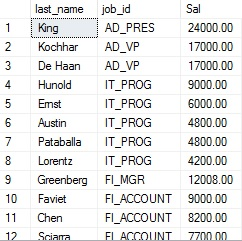
\includegraphics[width=5cm]{./Imagenes/actividad0101} 
	\end{center}

	\item SELECT * FROM job\_grades;
	\\Es incorrecta, la sentencia correcta sería:
	\\SELECT * FROM jobs;
	\begin{center}
	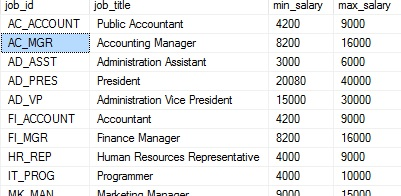
\includegraphics[width=5cm]{./Imagenes/actividad0102} 
	\end{center}
	
	\item SELECT employee\_id, last\_name sal x 12 ANNUAL SALARY FROM employees;
	\\Es incorrecta, la sentencia correcta sería:
	\\SELECT employee\_id, last\_name, salary * 12 'ANNUAL SALARY' FROM employees;
	\begin{center}
	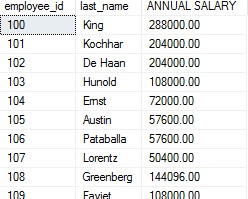
\includegraphics[width=5cm]{./Imagenes/actividad0103} 
	\end{center}

\end{itemize} 
\section{Actividad No 02 – Reconociendo la estructura} 

\begin{enumerate}[1.]
	\item Se requiere determinar la estructura de la tabla DEPARTMENTS y sus datos.
	\\
	\\SP\_HELP 'DEPARTMENTS'

	\begin{center}
	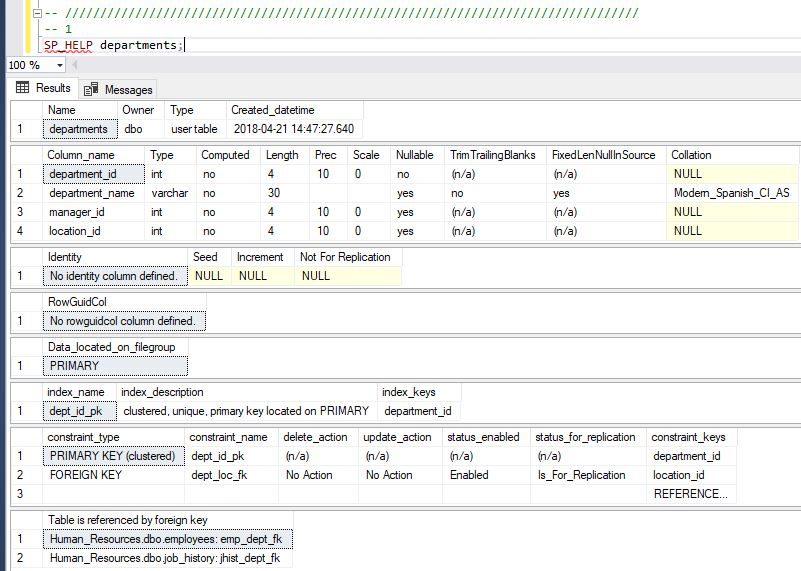
\includegraphics[width=10cm]{./Imagenes/actividad0201} 
	\end{center}

	\item El departamento de Recursos Humanos requiere un reporte que muestre los campos: employee\_id, last\_name y job\_id, asicomo el campo hire\_date con el alias StartDate.
	\\
	\\SELECT emp.employee\_id, \\
	emp.last\_name, \\
	emp.job\_id, \\
	emp.hire\_date AS StartDate \\
	FROM employees AS emp; 

	\begin{center}
	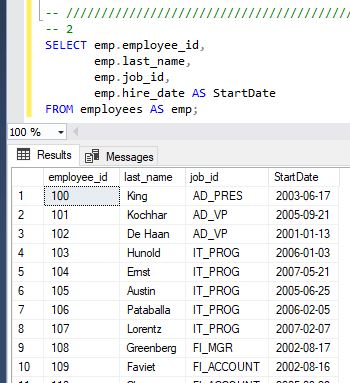
\includegraphics[width=5cm]{./Imagenes/actividad0202} 
	\end{center}

	\item Finalmente el departamento de Recursos Humanos requiere un listado de todos valores del campo JOB\_ID de la tabla EMPLOYEES pero que se muestren de forma única y no repetida.
	\\
	\\SELECT DISTINCT job\_id FROM employees; 

	\begin{center}
	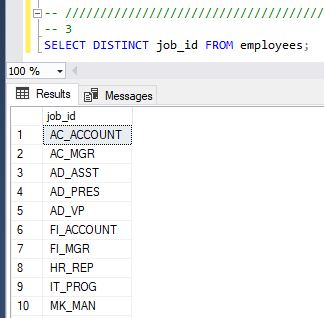
\includegraphics[width=5cm]{./Imagenes/actividad0203} 
	\end{center}

\end{enumerate}



\section{Actividad No 03 – Consultas B\'asicas} 
		
\begin{enumerate}[1.]
	\item El departamento de Recursos Humanos requiere ampliar el reporte anterior (4.2.2) para hacerlo m\'as comprensible, por lo que se requiere que los encabezados de las columnas sean: Emp No, Empleado, Puesto y Fecha Contrataci\'on.
	\\
	\\SELECT emp.employee\_id AS 'Emp N', \\
	   emp.last\_name AS Empleado, \\
	   emp.job\_id AS Puesto, \\
	   emp.hire\_date AS 'Fecha de contrataci\'on' \\
	FROM employees AS emp; \\
	\begin{center}
	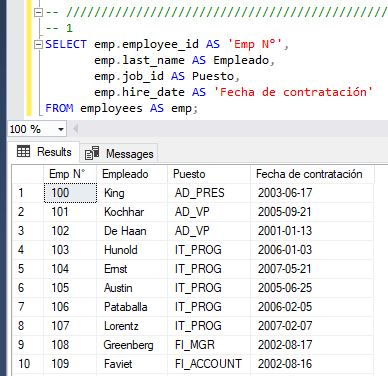
\includegraphics[width=5cm]{./Imagenes/actividad0301} 
	\end{center}

	\item Adicionalmente el departamento de Recursos Humanos requiere un reporte más sencillo, en el que se muestre los campos: last\_name y job\_id en una sola y \'unica columna (los datos deben estar separados por una coma) que tenga como alias Empleado y Puesto.
	\\
	\\SELECT CONCAT(emp.last\_name,',',emp.job\_id) AS 'Empleado y Puesto' \\
	\\FROM employees AS emp; \\
	\begin{center}
	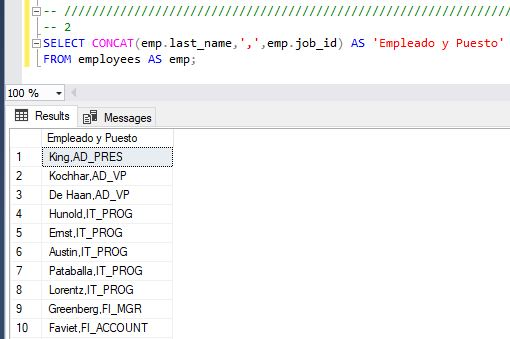
\includegraphics[width=5cm]{./Imagenes/actividad0302} 
	\end{center}

	\item  Finalmente a modo de práctica, realizar una consulta que muestre todos los campos de la tabla EMPLOYES, en una sola y única columna, los datos deben estar separado por una coma y la columna debe tener como encabezado Los Empleados
	\\
	\\SELECT CONCAT(emp.employee\_id,',', \\
			  emp.first\_name,',', \\
			  emp.last\_name,',', \\
			  emp.email,',', \\
			  emp.phone\_number,',', \\
			  emp.hire\_date,',', \\
			  emp.job\_id,',', \\
			  emp.salary,',', \\
			  emp.commission\_pct,',', \\
			  emp.manager\_id,',', \\
			  emp.department\_id) AS 'Los empleados' \\
	FROM employees AS emp; \\
	\begin{center}
	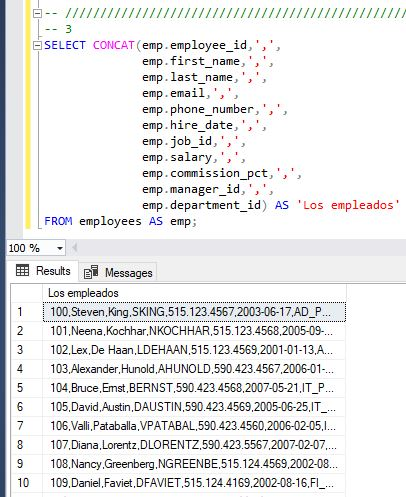
\includegraphics[width=5cm]{./Imagenes/actividad0303} 
	\end{center}

\end{enumerate}




\section{Actividad No 04 – Restricci\'on y Ordenamiento} 
		
\begin{enumerate}[1.]
	\item Debido a problemas con el presupuesto, el departamento de Recursos Humanos requiere un reporte que muestre los apellidos (last\_name) y salarios (salary) de todos los empleados que ganen más de \$ 12,000.
	\\ \\ select last\_name,salary from employees where salary > 12000;

	\begin{center}
	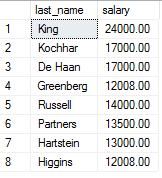
\includegraphics[width=5cm]{./Imagenes/actividad_04_01} 
	\end{center}

	\item Asimismo se requiere realizar una consulta que muestre los apellidos (last\_name) y el n\'umero de departamento (department\_id) para los empleados que tengan numero (employee\_id) 176.
	\\ \\select last\_name,department\_id from employees where employee\_id > 176;

	\begin{center}
	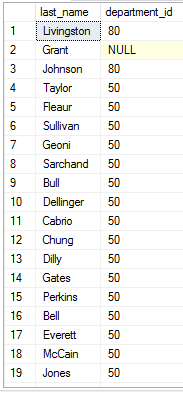
\includegraphics[width=5cm]{./Imagenes/actividad_04_02} 
	\end{center}

	\item El departamento de Recursos Humanos necesita determinar los mayores y menores sueldos, modificar la consulta del  ítem 4.1. para mostrar el apellido y salario de cada empleado cuyo sueldo no est\'e en el rango de \$ 5,000 a \$ 12,000.
	\\ \\select last\_name,job\_id,salary as Sal from employees where salary > 5000 and salary < 12000;

	\begin{center}
	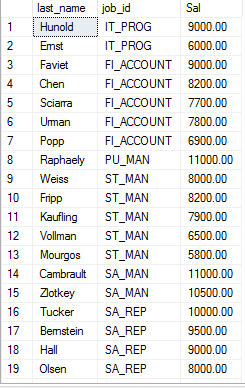
\includegraphics[width=5cm]{./Imagenes/actividad_04_03} 
	\end{center}

	\item Crear un reporte que muestre los apellidos (last\_name), puesto (job\_id) y fecha de contrataci\'on (hire\_date), de los empleados que apellidan ‘Matos’ y ‘Taylor’, asimismo presentar el reporte ordenado ascendentemente por fecha de contrataci\'on.
	\\ \\select last\_name,job\_id,hire\_date from employees where last\_name = 'Matos' or last\_name = 'Taylor' order by hire\_date asc;

	\begin{center}
	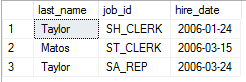
\includegraphics[width=5cm]{./Imagenes/actividad_04_04} 
	\end{center}

	\item Mostrar los apellidos (last\_name) y n\'umero de departamento (departamento\_id) de todos los empleados que pertenezcan a los departamentos 20 o 50 en orden alfab\'etico ascendente por el apellido.
	\\ \\select last\_name,department\_id from employees where department\_id = 20 or department\_id = 50 order by last\_name asc;
	
	\begin{center}
	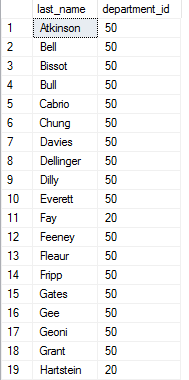
\includegraphics[width=5cm]{./Imagenes/actividad_04_05} 
	\end{center}
	
	\item Modificar el reporte del ítem 4.1. para mostrar los apellidos y salarios de los empleados que tengan un salario entre los \$ 5,000 a \$ 12,000 y pertenezcan a los números de departamento 20 o 50. Asimismo etiquetar las cabeceras de los resultados con los alias Empleado y Salario Mensual respectivamente.
	\\ \\select last\_name 'Empleado',salary 'Salario Mensual' from employees where salary > 5000 and salary < 12000 and (department\_id = 20 or department\_id = 50);

	\begin{center}
	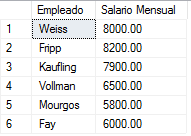
\includegraphics[width=5cm]{./Imagenes/actividad_04_06} 
	\end{center}

	\item El departamento de Recursos Humanos necesita un listado de apellidos (last\_name) y fecha de contrataci\'on (hire\_date) de todos los empleados que fueron contratados el año 1994.
	\\ \\select last\_name,hire\_date from employees where hire\_date between '19940101' and '19941231';

	\begin{center}
	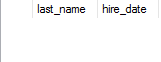
\includegraphics[width=5cm]{./Imagenes/actividad_04_07} 
	\end{center}

	\item Crear un reporte que muestre los apellidos (last\_name) y puesto (job\_id) de todos los empleados que no tengan un administrador (manager).
	\\ \\select last\_name,job\_id from employees where manager\_id is null;

	\begin{center}
	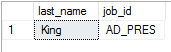
\includegraphics[width=5cm]{./Imagenes/actividad_04_08} 
	\end{center}

	\item Crear un reporte para mostrar los apellidos (last\_name), salario (salary) y \% de comisión (commission\_pct). Ordenar los datos por salario y comisión de manera descendente, utilizar la opción numérica de la cláusula ORDER BY.
	\\ \\select last\_name,salary,commission\_pct from employees order by salary desc,commission\_pct desc;

	\begin{center}
	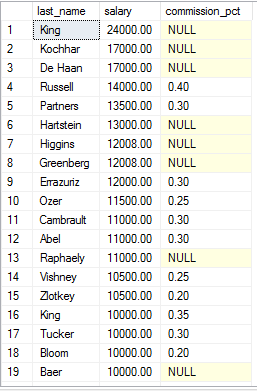
\includegraphics[width=5cm]{./Imagenes/actividad_04_09} 
	\end{center}


	\item El personal del departamento de Recursos Humanos desea tener mayor flexibilidad con los reportes hechos. Por ejemplo se requiere un reporte de los apellidos (last\_name) y salarios (salary) de todos los empleados que tengan un salario mayor a un monto que el personal de Recursos Humanos ingresará. Probar con el valor \$ 12,000.
	\\ \\declare @salario as decimal(9,2); set @salario = 12000; select last\_name,salary from employees where salary > @salario;

	\begin{center}
	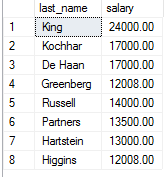
\includegraphics[width=5cm]{./Imagenes/actividad_04_10} 
	\end{center}

	\item El departamento de Recursos Humanos requiere extraer reporte basados en el Administrador (manager\_id). Se requiere crear una consulta que pregunte al usuario por el Administrador (manager\_id) y genere un reporte con los números de empleado (employee\_id), apellidos (last\_name), salarios (salary) y numero de departamento de los empleados que este Administrador tiene a su cargo. Adicionalmente también se desea tener la habilidad de ordenar este reporte en base a una determinada columna. Probar con los siguientes valores:
	\\Administrador (manager\_id) = 103, ordenado por Apellido (last\_name)
	\\Administrador (manager\_id) = 201, ordenado por Salario (salary)
	\\Administrador (manager\_id) = 124, ordenado por No de Empleado (employee\_id)
	\\ \\declare @gerente as int;
	\\set @gerente = 103;
	\\select employee\_id,last\_name,salary,department\_id from employees where manager\_id = @gerente order by last\_name;
	\\set @gerente = 201;
	\\select employee\_id,last\_name,salary,department\_id from employees where manager\_id = @gerente order by salary;
	\\set @gerente = 124;
	\\select employee\_id,last\_name,salary,department\_id from employees where manager\_id = @gerente order by employee\_id;
	\\go
	
	\begin{center}
	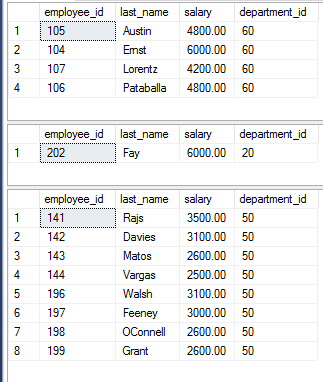
\includegraphics[width=5cm]{./Imagenes/actividad_04_11} 
	\end{center}

	\item Generar un listado de apellidos (last\_name) de todos los empleados que tengan la letra ‘a’ en la tercera letra de su apellido.
	\\ \\select last\_name from employees where SUBSTRING(last\_name,3,1) = 'a';
	\\go

	\begin{center}
	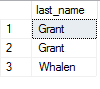
\includegraphics[width=5cm]{./Imagenes/actividad_04_12} 
	\end{center}

	\item Mostrar los apellidos (last\_name) de todos los empleados que tengan tanto la letra ‘a’ como la letra ‘e’ en su apellido.
	\\ \\select last\_name from employees where SUBSTRING(last\_name,3,1) = 'a' or SUBSTRING(last\_name,3,1) = 'e';
	\\go

	\begin{center}
	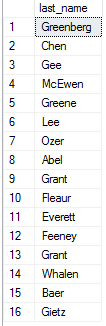
\includegraphics[width=5cm]{./Imagenes/actividad_04_13} 
	\end{center}

	\item Mostrar los apellidos (last\_name), puestos (job\_id) y salario (salary) de todos los empleados que sean Representantes de Ventas (SA\_REP) o Responsables de Inventario (ST\_CLERK) y cuyos salarios no sean iguales a \$ 2,500, \$ 3,500 o \$ 7,000.
	\\ \\select last\_name,job\_id,salary from employees where (job\_id = 'SA\_REP' or job\_id = 'ST\_CLERK') and (salary = 2500 or salary = 3500 or salary = 7000);
	\\go

	\begin{center}
	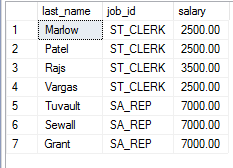
\includegraphics[width=5cm]{./Imagenes/actividad_04_14} 
	\end{center}

	\item Modificar el reporte del ítem 4.6 y mostrar adicionalmente los datos de comisión (commission\_pct) de todos los empleados que solamente el 20\% de comisi\'on.
	\\ \\select last\_name 'Empleado',salary 'Salario Mensual',commission\_pct from employees where salary > 5000 and salary < 12000 and (department\_id = 20 or department\_id = 50) and commission\_pct = 0.20;
	\\go

	\begin{center}
	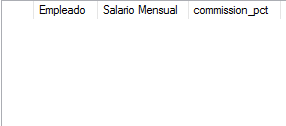
\includegraphics[width=5cm]{./Imagenes/actividad_04_15} 
	\end{center}

\end{enumerate}


\include{Secciones/Actividad05}
\include{Secciones/Actividad06}
\section{Actividad No 07 – Funciones de Agrupaci\'on} 
		
\begin{enumerate}[1.]
	\item El departamento de Recursos Humanos requiere un reporte que muestre el máximo, el mínimo, la suma y el promedio de los salarios de todos los empleados, Etiquetar esta columnas como Máximo, Mínimo, Suma y Promedio respectivamente, Redondear estos valores a enteros sin decimales.
	\\
	\\SELECT ROUND(MAX(salary),0) AS "Maximo" , ROUND(MIN(salary),0) AS "Minimo", ROUND(SUM(salary),0) AS "Sumatoria", ROUND(AVG(salary),0) AS "Promedio"
	\\FROM employees;
    	\begin{center}
	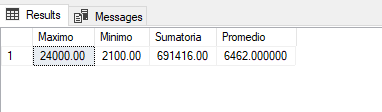
\includegraphics[width=5cm]{./Imagenes/Imagen01_Act07} 
	\end{center}
	\item Modificar la consulta anterior para mostrar el máximo, mínimo, suma y promedio de los salarios por cada Puesto de trabajo. 
	\item Realizar un reporte que muestre la cantidad de empleados por Puesto de trabajo. Con la opción de que el usuario pueda ingresar todos los puestos o uno solo.
	\\	
	\\SELECT COUNT(*)	
	\\FROM employees
	\\GROUP BY job\_id;
	\begin{center}
	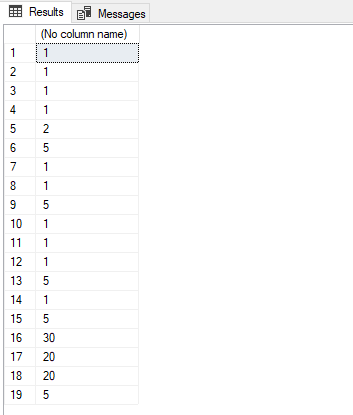
\includegraphics[width=5cm]{./Imagenes/Imagen02_Act07} 
	\end{center}
	\item Determinar el n\'umero de Administradores o Supervisores utilizar la columna manager\_id para esto. Etiquetar la columna como No de Administradores
	\\	
	\\SELECT COUNT(DISTINCT manager\_id) AS "Numero de Administradores"
	\\FROM employees;
	\begin{center}
	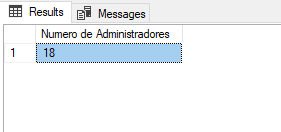
\includegraphics[width=5cm]{./Imagenes/Imagen03_Act07} 
	\end{center}
	\item Encontrar la diferencia entre el m\'aximo y m\'inimo salario de los empleados. Etiquetar la columna como Diferencia
	\\
	\\SELECT (MAX(salary) - MIN(salary)) AS "diferencia"
	\\FROM employees;
	\begin{center}
	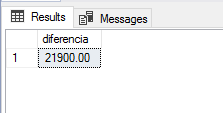
\includegraphics[width=5cm]{./Imagenes/a7a5} 
	\end{center}
	\item Crear un reporte que muestre los No de Administradores (manager\_id) y el salario de su empleado peor pagado. Excluir a los empleados cuyo Administrador no se conozca. Excluir asimismo cualquier grupo cuyo salario mínimo sea \$6000 o menos. Ordenar los resultados por el mínimo salario en forma descendente.
	\\
	\\SELECT salman.minimo,
	\\salman.manager\_id
	\\FROM (SELECT MIN(salary) AS 'minimo',
	\\manager\_id
	\\FROM employees
	\\WHERE salary>6000
	\\GROUP BY manager\_id) AS salman
	\\ORDER BY salman.minimo;
	\begin{center}
	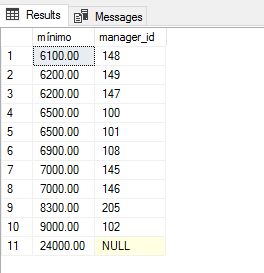
\includegraphics[width=5cm]{./Imagenes/a7a6} 
	\end{center}
	\item Crear una consulta que muestre el número total de empleados, así como el número total de empleados contratados en los años 1995, 1996, 1997 y 1998, etiquetar las columnas apropiadamente.
	\item Crear una consulta matriz que muestre el puesto, el salario por cada puesto basado en el No de Departamento del empleado y el total del salario para cada puesto para los departamento 20, 50, 80 y 90, colocar un nombre apropiado a cada columna.
\end{enumerate}


\section{Actividad No 08 – Enlaces} 
		
\begin{enumerate}[1.]
	\item El departamento de Recursos Humanos requiere un reporte que muestre las direcciones de todos los departamentos. Utilizar las tablas LOCATIONS y COUNTRIES. Mostrar el ID de la Ubicación (location\_id), dirección (street\_address), ciudad (city), estado o provincia (state\_province) y país (country\_name). % Utilizar NATURAL JOIN para producir el resultado.
	\\
	\\select l.location\_id , l.street\_address , l.city , l.state\_province , c.country\_name 
	\\from locations as l 
	\\join countries as c 
	\\on l.country\_id = c.country\_id

	\begin{center}
	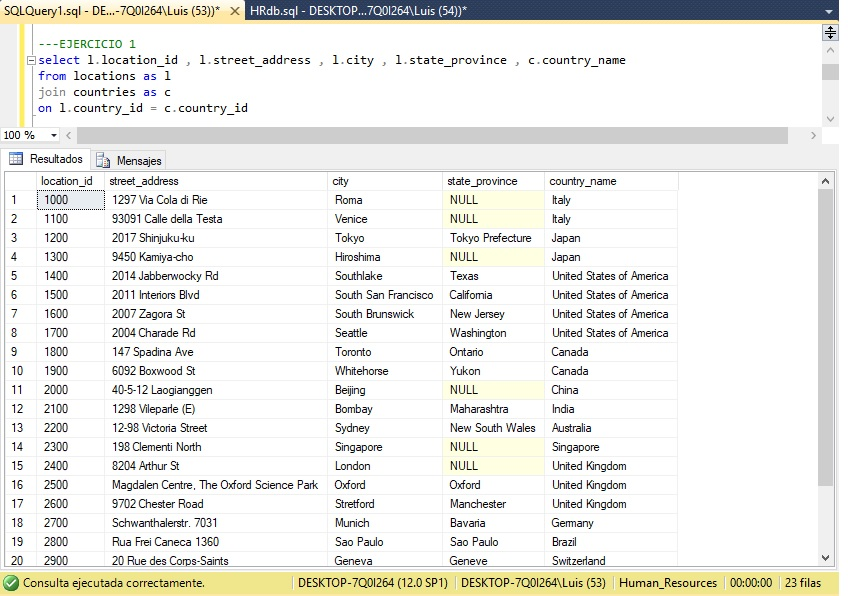
\includegraphics[width=5cm]{./Imagenes/8ejer1} 
	\end{center}


	\item El departamento de Recursos Humanos necesita un reporte de todos empleados, que muestres los apellidos de empleado (last\_name), el No de departamento (department\_id) y el nombre del departamento (depertment\_date) al cual pertenece. 
	\\
	\\select e.last\_name , d.department\_id , d.department\_name from employees as e
	\\left join departments as d 
	\\on e.department\_id = d.department\_id order by d.department\_name;

	\begin{center}
	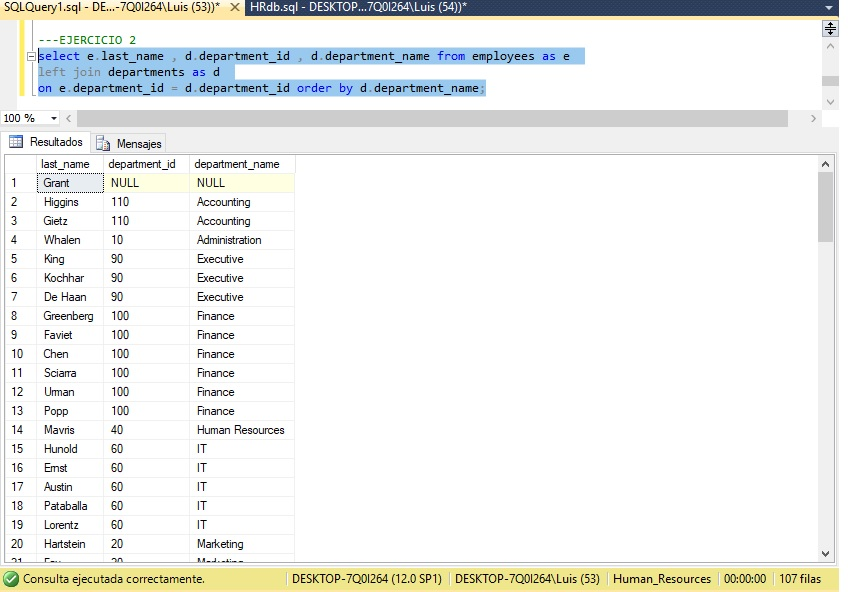
\includegraphics[width=5cm]{./Imagenes/8ejer2} 
	\end{center}

	\item El departamento de Recursos Humanos necesita un reporte de los empleados de la ciudad de Toronto. Mostrar los Apellidos, Puesto, No de Departamento y Nombre de Departamento de todos los empleados que trabajan en Toronto.
	\\
	\\select e.last\_name , e.department\_id, j.job\_title, d.department\_name , l.city 
	\\from employees as e 
	\\left join jobs as j 
	\\on e.job\_id = j.job\_id
	\\join departments as d
	\\on e.department\_id=d.department\_id
	\\join locations as l 
	\\on d.location\_id = l.location\_id
	\\where l.city='Toronto';

	\begin{center}
	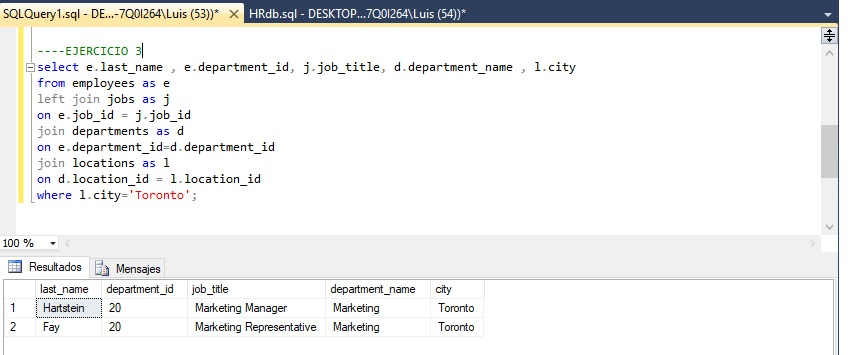
\includegraphics[width=5cm]{./Imagenes/8ejer3} 
	\end{center}

	\item Crear un reporte que muestre los Apellidos y No de Identificación de los empleados, asimismo también debe mostrarse el Apellido y No de Identificaci\'on de su Administrador.
	\\
	\\SELECT e.employee\_id 'ID\_Empleado', e.last\_name 'Empleado', 
	\\m.employee\_id 'ID\_Manager', m.last\_name 'Manager' 
	\\FROM employees e 
	\\join employees m 
	\\ON (e.manager\_id = m.employee\_id)


	\begin{center}
	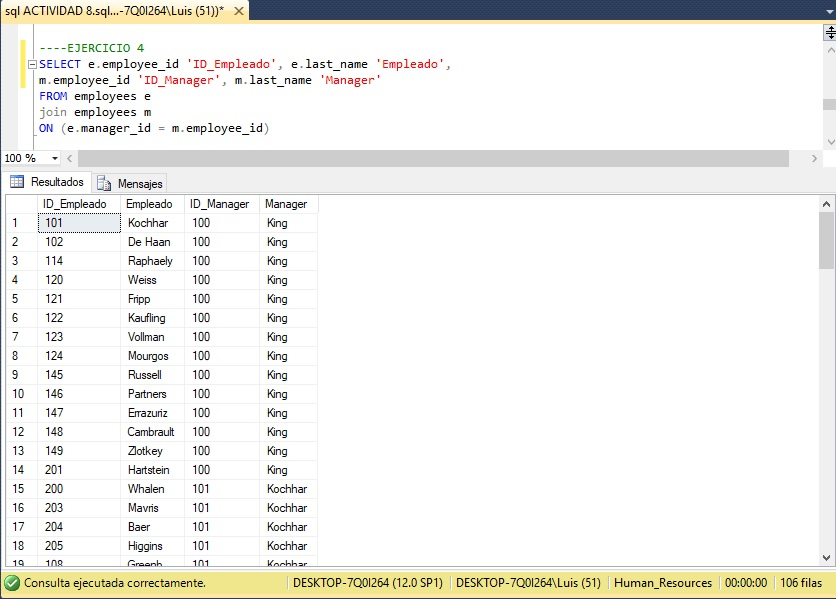
\includegraphics[width=5cm]{./Imagenes/8ejer4} 
	\end{center}

	\item Modificar la consulta anterior para que incluya tambi\'en a los empleados quienes no tienen Administrador asignado.
	\\
	\\SELECT e.employee\_id 'ID\_Empleado', e.last\_name 'Empleado', 
	\\m.employee\_id 'ID\_Manager', m.last\_name 'Manager' 
	\\FROM employees e 
	\\left outer join employees m
	\\ON (e.manager\_id = m.employee\_id)

	\begin{center}
	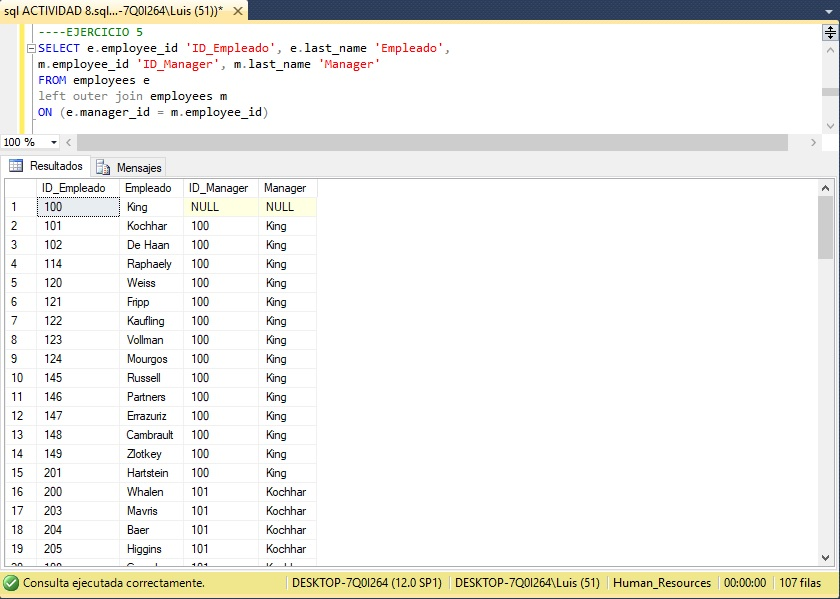
\includegraphics[width=5cm]{./Imagenes/8ejer5} 
	\end{center}

	\item Crear un reporte que muestre los No de Departamento y Apellidos de todos los empleados, asimismo adicionar una columna con los Apellidos de todos empleados que trabajan en el mismo departamento. Etiquetar esta columna como Colega.
	\\
	\\select e.department\_id 'DEPARTMENTO', e.last\_name 'EMPLEADO', 
	\\d.last\_name 'COLEGA' 
	\\from employees e 
	\\join employees d 
	\\on (e.department\_id=d.department\_id) and e.last\_name!=d.last\_name;\\

	\begin{center}
	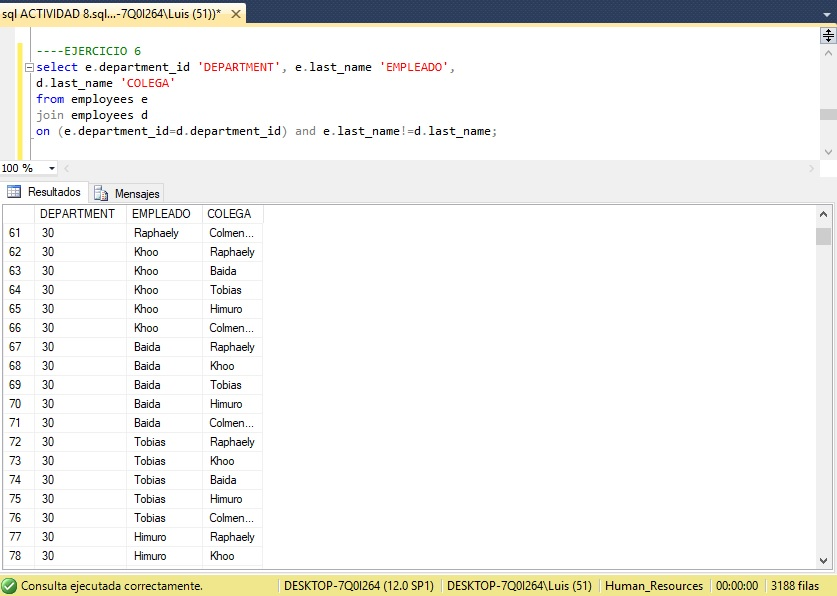
\includegraphics[width=5cm]{./Imagenes/8ejer6} 
	\end{center}

	\item El departamento de Recursos Humanos requiere un reporte de todo el personal que fue contratado después del empleado apellidado ‘Davies’. Crear un reporte que muestre el apellidos y fecha de contrataci\'on de todo los empleados contratado después de ‘Davies’.
	\\
	\\SELECT e.first\_name, e.last\_name, e.hire\_date 
	\\FROM employees e 
	\\JOIN employees davies 
	\\ON (davies.last\_name = 'Davies') 
	\\WHERE davies.hire\_date < e.hire\_date;

	\begin{center}
	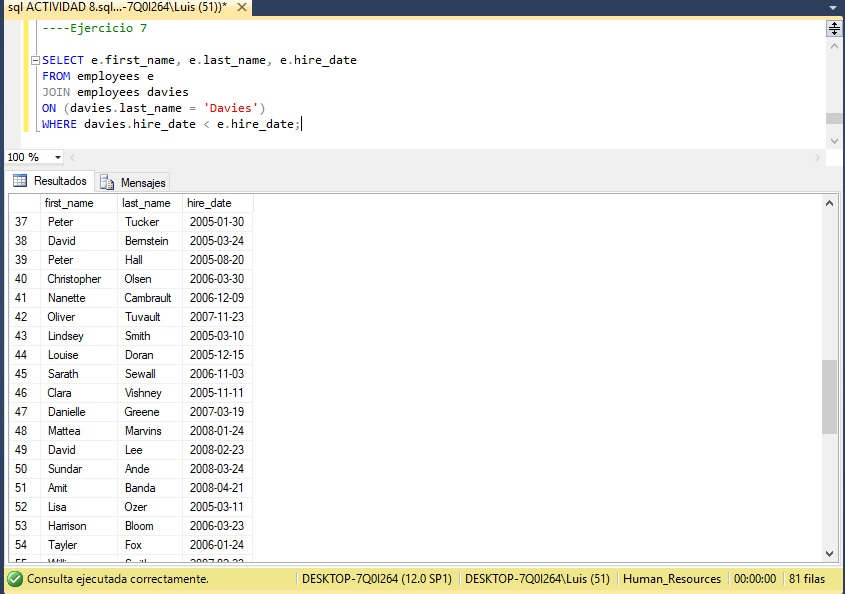
\includegraphics[width=5cm]{./Imagenes/8ejer7} 
	\end{center}


	\item El departamento de Recursos Humanos requiere de un reporte que el apellido del empleado, fecha de contrataci\'on del empleado, apellido del administrador, fecha de contratación del administrador. Para todos aquellos empleados que fueron contratados antes que sus Administradores.
	\\
	\\select e.last\_name 'EMPLEADO', e.hire\_date 'FECHA\_CONTRATACION' , j.last\_name 'ADMINISTRADOR', 
	\\j.hire\_date 'FECHA\_CONTRATACION\_ADMINISTRADOR'
	\\from employees e 
	\\join employees j 
	\\on e.manager\_id=j.employee\_id 
	\\and e.hire\_date < j.hire\_date 
	\\order by e.hire\_date;

	\begin{center}
	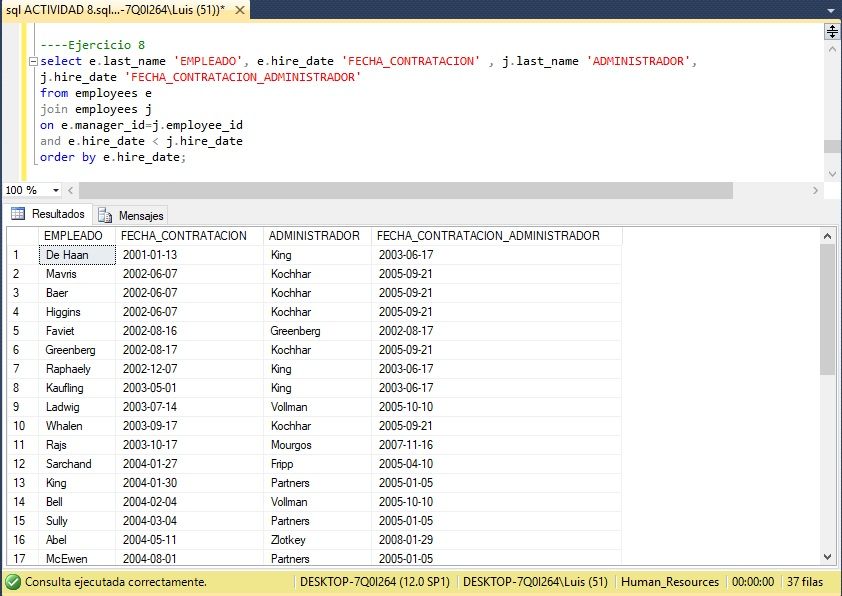
\includegraphics[width=5cm]{./Imagenes/8ejer8} 
	\end{center}

	\end{enumerate}
	



\section{Actividad No 09 – SubConsultas} 
		
\begin{enumerate}[1.]
	\item El departamento de Recursos Humanos requiere una consulta que pregunte al usuario por el Apellido del empleado, Luego la consulta deber\'a mostrar los Apellidos y Fecha de Contrataci\'on de todos los empleados del mismo departamento excluyendo o con excepción del empleado el cual ha sido proporcionado su apellido reporte que muestre las direcciones de todos los departamentos.
	\\
	\\-- leyendo id de empleado\\
	SET @empid \= 110\\
	-- obteniendo id de departamento de empleado \\
	SET @depid \= (SELECT emp.department\_id \\
	FROM employees as emp \\
	WHERE emp.employee\_id\=@empid); \\
	-- todos los empleados del mismo departamento excluyendo al empleado ingresado anteriormente\\
	SELECT emp.employee\_id, \\
	emp.last\_name, \\
	emp.hire\_date, \\
	emp.department\_id \\
	FROM employees AS emp \\
	WHERE emp.department\_id\=@depid \\
	AND emp.employee\_id!\=@empid; \\
	\begin{center}
	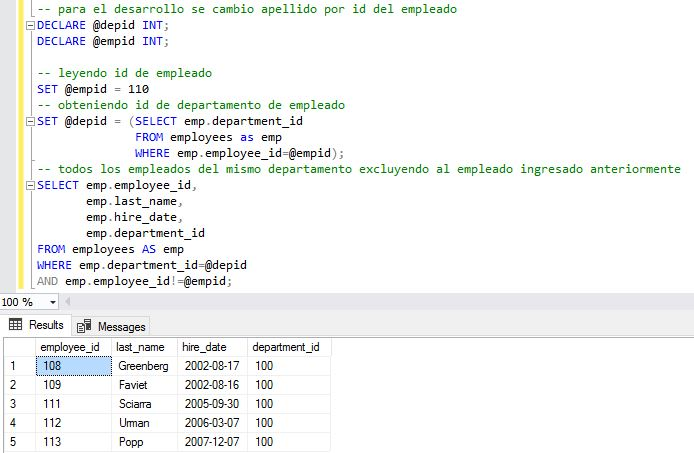
\includegraphics[width=5cm]{./Imagenes/actividad0901} 
	\end{center}

	\item Crear un reporte que muestre el No del Empleado, Apellidos y Salarios de todos los empleados que tienen un salario superior al promedio de salarios de todos los empleados. Ordenar los resultados por el Salario de forma ascendente.
	\\
	\\SELECT emp.employee\_id, \\
	emp.last\_name, \\
	emp.salary \\
	FROM employees AS emp \\
	WHERE emp.salary>@prom; \\
	\begin{center}
	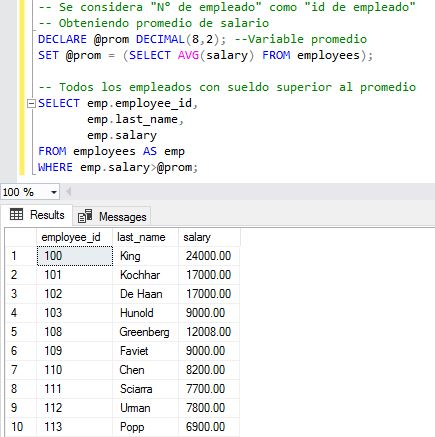
\includegraphics[width=5cm]{./Imagenes/actividad0902} 
	\end{center}

	\item Realizar un reporte que muestre el No de Empleado y Apellidos de todos los empleados quienes trabajan en el departamento de cualquier empleado que su apellido contenga la letra ‘u’.
	\\
	\\SELECT emp.employee\_id, \\
	emp.last\_name, \\
	emp.department\_id \\
	FROM employees AS emp \\
	JOIN (SELECT DISTINCT department\_id \\
		  FROM employees \\
		  WHERE last\_name LIKE '\%u\%') AS depid \\
	ON emp.department\_id\=depid.department\_id; \\
	\begin{center}
	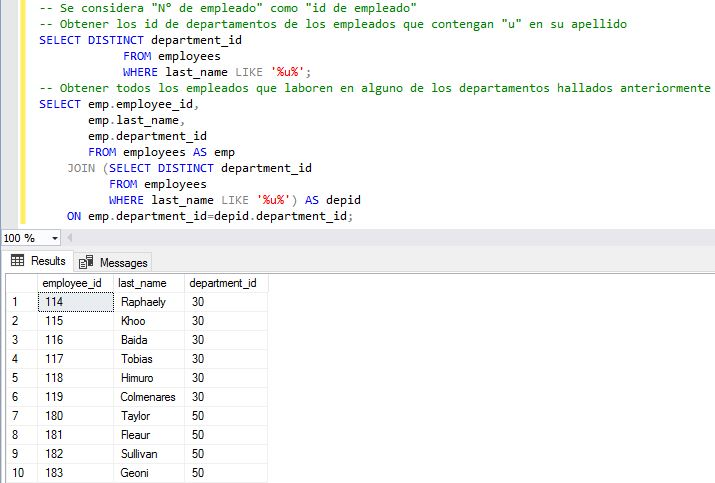
\includegraphics[width=5cm]{./Imagenes/actividad0903} 
	\end{center}

	\item El departamento de Recursos Humanos requiere un reporte que muestre los Apellidos, No de Departamento y Puestos de los empleados cuya locación de departamento es 1700.
	\\
	\\SELECT emp.last\_name, \\
	emp.department\_id, \\
	dep.location\_id \\
	FROM employees as emp \\
	JOIN departments as dep \\
	ON emp.department\_id\=dep.department\_id \\
	WHERE dep.location\_id\=1700;\\
	\begin{center}
	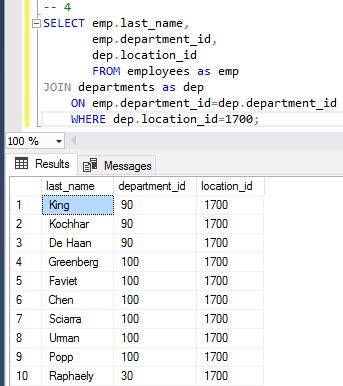
\includegraphics[width=5cm]{./Imagenes/actividad0904} 
	\end{center}

	\item Modificar la consulta anterior de forma que el usuario pueda introducir el No de locaci\'on.
	\\
	\\DECLARE @locid INT; \\
	SET @locid \= 1700; \\
	SELECT emp.last\_name, \\
	   emp.department\_id, \\
	   dep.location\_id \\
	   FROM employees as emp \\
	JOIN departments as dep \\
	ON emp.department\_id\=dep.department\_id \\
	WHERE dep.location\_id\=@locid; \\
	\begin{center}
	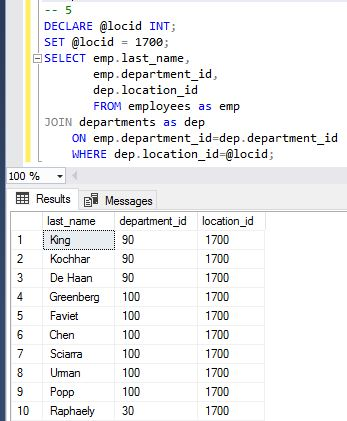
\includegraphics[width=5cm]{./Imagenes/actividad0905} 
	\end{center}

	\item Crear un reporte para el departamento de Recursos Humanos que muestre los Apellidos y Salarios de todos los empleados cuyo Administrador apellide ‘King’.
	\\
	\\SELECT emp.last\_name, \\
	   emp.salary \\
	   FROM employees AS emp \\
	JOIN (SELECT dep.department\_id \\
			 FROM departments AS dep \\
	  JOIN (SELECT employee\_id, \\
			       last\_name \\
				   FROM employees \\
				   WHERE last\_name\='KING') AS manking \\
	  ON dep.manager\_id\=manking.employee\_id) AS depking \\
	ON emp.department\_id\=depking.department\_id; \\
	\begin{center}
	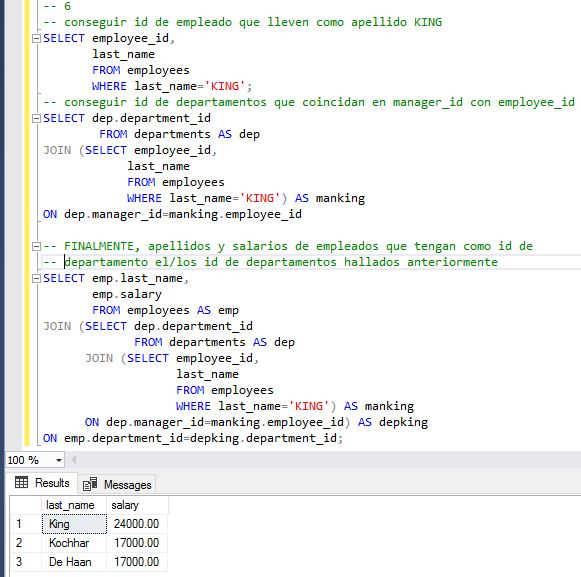
\includegraphics[width=5cm]{./Imagenes/actividad0906} 
	\end{center}

	\item Crear un reporte para el departamento de Recursos Humanos que muestre el No de Departamento, Apellidos, Puestos de todos los empleados en el departamento ‘Executive’.
	\\
	\\SELECT empnomjob.department\_id, \\
	   empnomjob.last\_name, \\
	   empnomjob.job\_title \\
	   FROM departments \\
	JOIN (SELECT emp.department\_id, \\
			 emp.last\_name, \\
			 jobs.job\_title \\
			 FROM employees AS emp \\
	  JOIN jobs \\
	  ON emp.job\_id\=jobs.job\_id) AS empnomjob \\
	ON empnomjob.department\_id\=departments.department\_id \\
	WHERE department\_name\='executive' \\

	\begin{center}
	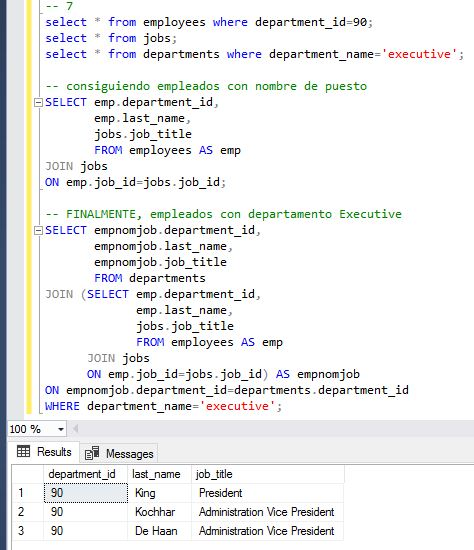
\includegraphics[width=5cm]{./Imagenes/actividad0907} 
	\end{center}

	\item Modificar la consulta del ítem 4.3 para que adicionalmente se muestro solo a los empleados que tengan un salario mayor al promedio de todos los salarios de los empleados.



\end{enumerate}

\section{Actividad No 10 – Conjuntos} 
		


\begin{enumerate}[1.]
	\item El departamento de Recursos Humanos requiere un reporte de todos los departamentos que no contengan un empleado con el puesto ‘ST\_CLERK’. Utilizar el operador MINUS o EXCEPT para esta solicitud.
	\\
	\\select department\_id from employees
	\\where job\_id ='ST\_CLERK';

	\begin{center}
	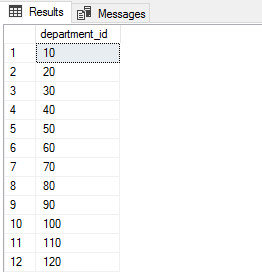
\includegraphics[width=5cm]{./Imagenes/ejercicio10-1} 
	\end{center}

	\item El departamento de Recursos Humanos requiere adicionalmente una lista de todos los pa\'ises que no tengan un departamento de la empresa localizado en ellos, mostrar el código del país y el nombre. Utilizar el operador MINUS o EXCEPT para realizar esta operaci\'on.
	\\
	\\select county\_id, country\_name from countries
	\\minus

	\begin{center}
	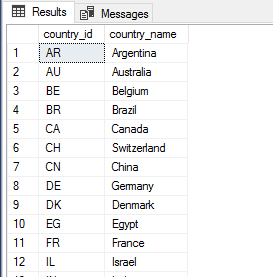
\includegraphics[width=5cm]{./Imagenes/ejercicio10-2} 
	\end{center}

	\item Se necesita una lista de puestos de los departamentos 10, 50 y 20, en ese orden, mostrar el c\'odigo del puesto y c\'odigo del departamento. Utilizar el operador UNION ALL.
	\\
	\\select distinct job\_id, department\_id from employees
	\\where (department\_id=10) 	
	\\union
	\\select distinct job\_id, department\_id from employees
	\\where (department\_id=50)
	\\union
	\\select distinct job\_id, department\_id from employees
	\\where  (department\_id=20);

	\begin{center}
	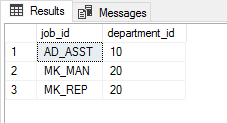
\includegraphics[width=5cm]{./Imagenes/ejercicio10-3} 
	\end{center}

	\item Crear un reporte que muestre que liste los c\'odigos de los empleados y los puestos de todos aquellos empleados que tienen el mismo puesto que en el momento en el que fueron contratados por la empresa, cambiaron de puestos y luego volvieron al puesto anterior. Utilizar el operador INTERSECT.
	\\
	\\select employee\_id, job\_id from employees
	\\intersect
	\\select distinct employee\_id, job\_id from job\_history;

	\begin{center}
	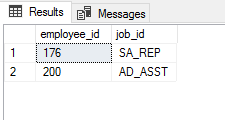
\includegraphics[width=5cm]{./Imagenes/ejercicio10-4} 
	\end{center}

	\item El departamento de Recursos Humanos requiere un reporte que muestre lo siguiente:

	\begin{itemize}
		\item Apellidos y c\'odigos de departamentos de todos los registros de la tabla empleados sin importar si pertenecen a uno o ningún departamento.
		\item C\'odigo de departamentos y nombres de departamentos de la tabla DEPARTAMENTOS inclusive si no existiese ningún empleado en ese departamento
	\end{itemize}
	Ambos requerimientos se deben mostrar en un mismo resultado. Utilizar el operador UNION ALL.
	\\
	\\select last\_name, department\_id, null from employees union select null, department\_id, department\_name from departments;

	\begin{center}
	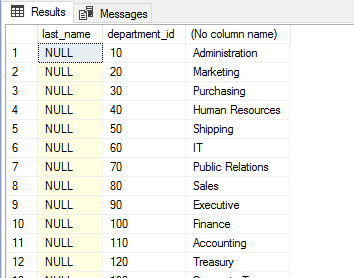
\includegraphics[width=5cm]{./Imagenes/ejercicio10-5} 
	\end{center}

\end{enumerate}

\end{document}
